\documentclass[22pt]{beamer}
\usepackage[orientation=portrait, size=custom, width=91.44, height=91.44,scale=1.2]{beamerposter} % 36in*2.5 = 90cm
\usepackage[absolute,overlay]{textpos}
\usepackage{bookmark} %pdflatex says to use this to avoid errors...
\usepackage{graphicx} %for including images
\graphicspath{{assets/images/}} %location of images
\usepackage{wrapfig} %wrap text around the images
\usepackage{listingsutf8}    %package for code environment; use this instead of verbatim to get automatic line break; use this instead of listings to get (•)
\usepackage{amsmath}
\usepackage{gensymb}
\usepackage[export]{adjustbox}
\usepackage[skins,theorems]{tcolorbox}
\usepackage{tikz}
\newcommand*\circled[1]{\tikz[baseline=(char.base)]{
            \node[shape=circle,draw,inner sep=2pt] (char) {#1};}}
\usepackage{array}
\usepackage{booktabs,adjustbox}
\usepackage{subcaption}
\usepackage{pgfplots}
%plot options
\pgfplotsset{width=7cm,compat=1.8}
\PassOptionsToPackage{gray}{xcolor}
\usepackage{cite}
\usepackage{fancyvrb}

\usetikzlibrary{shapes,shapes.geometric,arrows,fit,calc,positioning,automata,}
\usepackage{pgf-pie}

\usepackage{wrapfig}

%\mode<presentation>
%this doesn't seem to make any difference; leave for now for trying out
\usetheme{Berlin}
\definecolor{MacBlue}{rgb}{0.10196,0.22353,0.53725}
\definecolor{MacMaroon} {rgb}{0.47843, 0, 0.23137}
\definecolor{MacMaroon2} {rgb}{0.47451, 0, 0}
\definecolor{MacGray}{rgb}{0.50196,0.49804,0.51765}
\definecolor{MacMaroon3}{rgb}{00.47,0.2,0.31}
\definecolor{MacGold}{rgb}{1, 0.75,0.35}
\usecolortheme[named=MacMaroon2]{structure}
\setbeamertemplate{caption}[numbered]
\setbeamertemplate{navigation symbols}{}

% From https://tex.stackexchange.com/questions/201216/beamer-nested-lists-do-not-decrease-the-font-size
\setbeamerfont{itemize/enumerate subbody}{size=\normalsize} %to set sub-itemize size

\title{A New Taxonomy of Software Testing Approaches}
\subtitle{Seeking More Standardized Standards}
  \author[Crawford, Carette, \& Smith]{Samuel Joseph Crawford, Jacques Carette, \& Spencer Smith\newline \small \{crawfs1, carette, smiths\}@mcmaster.ca}
  \institute[McMaster University]{Department of Computing and Software, McMaster University} % $^\dagger$
  \date{April 22, 2023}

\begin{document}
%compile with pdflatex

%there is only one frame, because there is only one page; yeah, it's a poster
%textblock and block seem to work nicely to organize layout
\begin{frame}[fragile]

    \begin{textblock}{2}(0.7,1)
        
\includegraphics[height=8.5cm]{eng_logo.png}
    \end{textblock}

    \begin{textblock}{2}(13,0.55)
        
\includegraphics[height=12.5cm]{cas_logo.png}
    \end{textblock}

    \begin{textblock}{8}(4,1)
        \titlepage
    \end{textblock}

    \begin{textblock}{7.25}(0.5,2.75)

        %this needs help
        \begin{block}{\fontsize{37}{20}\selectfont Goal}
            The first step to any formal process is \textbf{understanding the
                underlying domain}. Therefore, a systematic and rigorous
            understanding of software testing approaches is needed to develop formal
            tools to test software. In our specific case, our motivation was seeing
            \textbf{which kinds of testing can be generated automatically by Drasil},
            ``a framework for generating all of the software artifacts for
            (well understood) research software'' \cite{carette_drasil_2021}.
            \vspace{7mm}
        \end{block}

        \begin{block}{\fontsize{37}{20}\selectfont Problem}
            Most software testing ontologies seem to focus on the high-level
            testing process rather than the testing approaches themselves. For
            example:
            \begin{itemize}
                \item Tebes et al.~(2020) mainly focus on parts of the
                      testing process (e.g., test goal, testable entity)
                \item Unterkalmsteiner et al.~(2014) provide a foundation for
                      classification but not its results
                      %   ``do[] not aim at providing a systematic
                      %   and exhaustive state-of-the-art survey of [either domain]''
                      %   (p.~A:2)
            \end{itemize}
            \vspace{5mm}
        \end{block}

        \begin{block}{\fontsize{37}{20}\selectfont Methodology}
            Since a taxonomy doesn't already exist, we should create one!
            \begin{itemize}
                \item We started with an ad hoc approach, focusing on
                      textbooks \textbf{trusted at McMaster University}
                      %   \\\cite{Patton2006,
                      %       PetersAndPedrycz2000, vanVliet2000}
                \item We then realized that this was too arbitrary, so
                      we started from \textbf{more established sources}, such as
                      IEEE and SWEBOK
                      %   \\\cite{IEEE2022, SWEBOK2024, SWEBOK2014,
                      %       IEEE2017, ISO_IEC2023a, ISTQB}
                \item The goal of this approach is to iterate,
                      eventually revisiting the original textbooks,
                      until enough knowledge is built up to encounter
                      diminishing returns (ideally no returns!)
                \item Since there are many standardized documents about software
                      testing (or software in general), \textbf{this should be
                          trivial, no?}
            \end{itemize}
            \vspace{5mm}
        \end{block}

        \begin{block}{\fontsize{37}{20}\selectfont In Our Experience}
            \vspace{5mm}
            \begin{center}
                {\fontsize{185}{20}\selectfont \textbf{NO.}}
            \end{center}
            \begin{columns}
                \begin{column}{0.7\textwidth}
                    \begin{center}
                        \begin{figure}
                            \centering
                            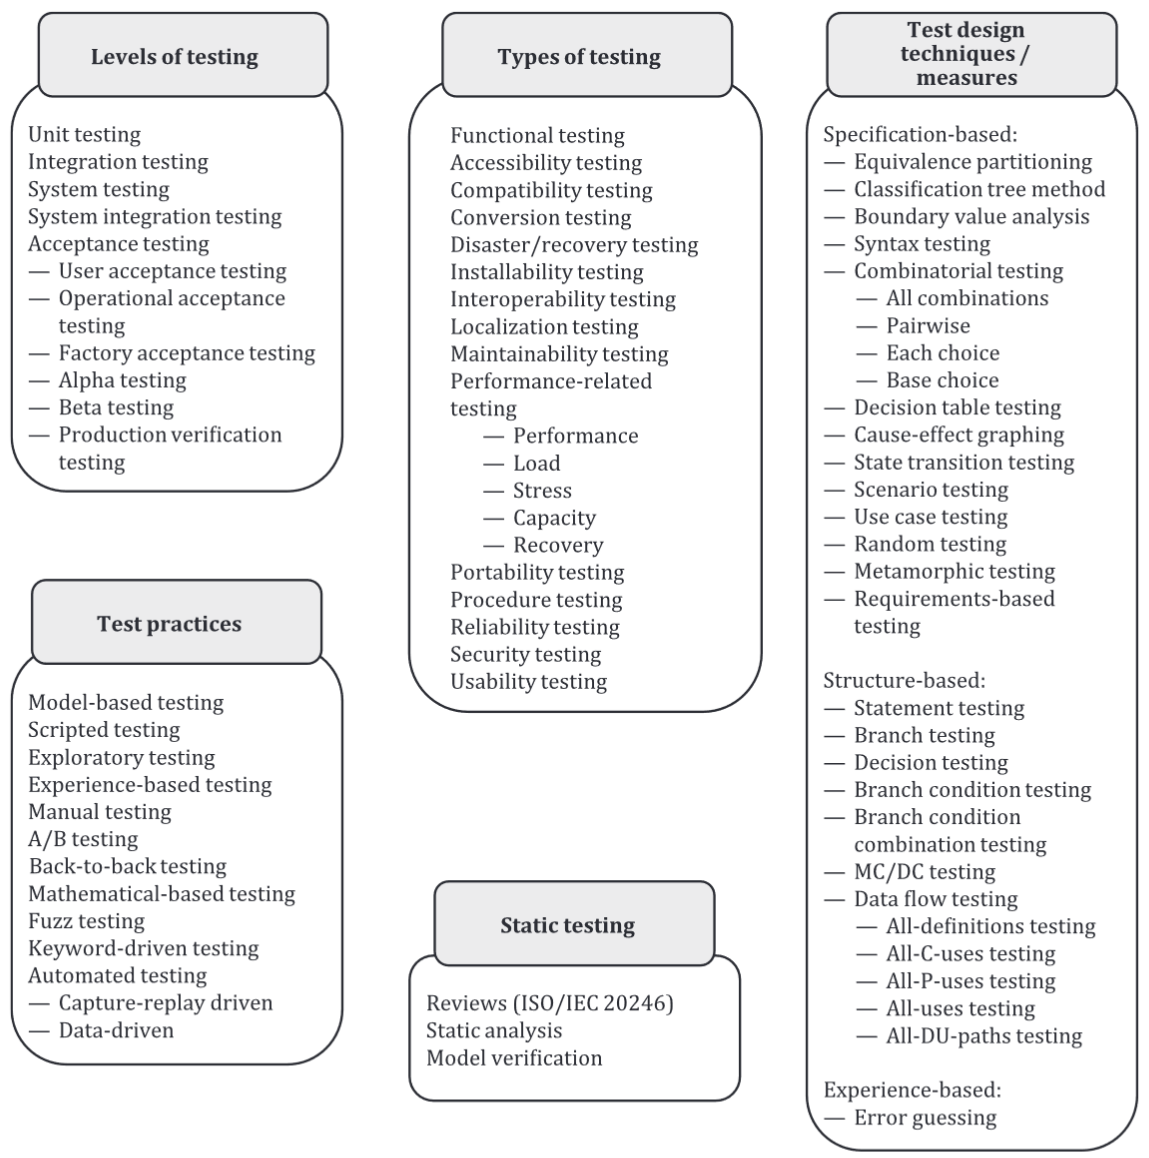
\includegraphics[width=\textwidth]{test approach choices.png}
                            \vspace{-5mm}
                            \caption{A classification of some ``test approach choices''
                                \cite[p.~22]{IEEE2022}.}
                            \label{Fig:approach-choices}
                        \end{figure}
                    \end{center}
                \end{column}
                \begin{column}{0.25\textwidth}
                    Information often \textbf{appears} logical, but this often
                    breaks down. For example, the classification of test
                    approaches in Figure~\ref{Fig:approach-choices} reveals the
                    following ambiguities:
                    \begin{itemize}
                        \item Experience-based testing is both a test design
                              technique \textbf{and} a test practice
                        \item What distinguishes the following pairs is unclear:
                              \begin{itemize}
                                  \item Disaster/recovery testing and recovery
                                        testing
                                  \item Branch condition testing and branch
                                        condition combination testing
                                        %   \item Operational acceptance testing and
                                        %         operational testing \cite[p.~303]{IEEE2017}
                              \end{itemize}
                    \end{itemize}
                \end{column}
            \end{columns}
            \vspace{3mm}
        \end{block}
    \end{textblock}

    \begin{textblock}{7.25}(8.25,2.75)
        \begin{block}{\fontsize{37}{20}\selectfont More Examples}
            A big contributor to the ambiguities in
            Figure~\ref{Fig:approach-choices} is the number of definitions that
            are not given. Despite its source \cite{IEEE2022} being a standard
            for general concepts related to software testing, it leaves much
            unstandardized. For example, as shown in Figure~\ref{Fig:IEEEdefs},
            most (55 out of 99) testing approaches mentioned \textbf{do not
                have a definition}! Eight of these were at the very least
            described in the previous version of this standard \cite{IEEE2013},
            and nine were present in the same way in another
            IEEE standard \cite{IEEE2017} that would have been available
            upon publication of this one. However, the presence of a
            definition does not guarantee that it is useful! See
            Figure~\ref{Fig:unhelpful-defs} for some good (bad?) examples.
            \vspace{-1cm}
            \begin{columns}
                \begin{column}{0.4\textwidth}
                    \begin{center}
                        \begin{figure}
                            \begin{tikzpicture}[thick, scale=1.5, every node/.style={align=left, scale=0.8}]
                                \pie{44.4/Defined,
                                38.4/Undefined,
                                9.1/{Present in\\another standard},
                                8.1/{Present in\\previous version}}
                            \end{tikzpicture}
                            \caption{Breakdown of testing approach definitions
                                from \cite{IEEE2022}.}
                            \label{Fig:IEEEdefs}
                        \end{figure}
                    \end{center}
                \end{column}
                \begin{column}{0.475\textwidth}
                    \begin{center}
                        \begin{figure}
                            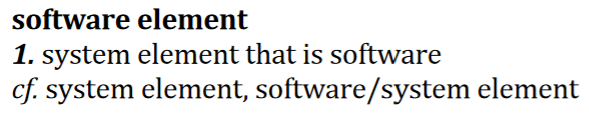
\includegraphics[width=\textwidth]{software element.png}

                            \vspace{2mm}

                            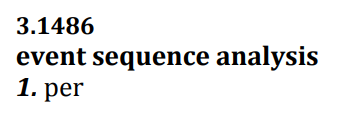
\includegraphics[height=3.9cm]{per.png}
                            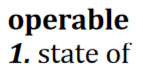
\includegraphics[height=3.8cm]{state of.png}
                            \caption{Some less-than-helpful definitions from
                                \cite[pp.~421, 170, 301, counterclockwise from top]{IEEE2017}.}
                            \label{Fig:unhelpful-defs}
                        \end{figure}
                    \end{center}
                \end{column}
            \end{columns}

            \quad\\ % needed for line break

            This problem also extends to definitions of software testing
            approaches. For example, SWEBOK V4 says ``scalability testing
            evaluates the capability to use and learn the system and the user
            documentation. It also focuses on the system's effectiveness in
            supporting user tasks and the ability to recover from user errors''
            \cite[p.~5-9]{SWEBOK2024}. This definition seems to be an
            amalgamation of the definitions of usability, recovery, and
            potentially functional testing. What's more, SWEBOK's definition
            of elasticity testing cites only one source \cite[p.~5-9]{SWEBOK2024};
            \textbf{one that doesn't contain the words ``elasticity'' or ``elastic''}!
            \vspace{5mm}\\
            Even when the general idea behind an approach is understood,
            discrepancies can still arise. While alpha testing is quite common
            and understood, there is disagreement on who performs it:
            \begin{enumerate}
                \item ``users within the organization developing the software''
                      \cite[p.~17]{IEEE2017},
                \item ``a small, selected group of potential users''
                      \cite[p.~5-8]{SWEBOK2024}, or
                \item ``roles outside the development organization''
                      \cite{ISTQB}
            \end{enumerate}
            \vspace{5mm}
        \end{block}

        \begin{block}{\fontsize{37}{20}\selectfont Conclusions \& Future Work}
            \begin{itemize}
                \item Current software testing taxonomies are \textbf{incomplete,
                          inconsistent, and/or incorrect}
                \item For one to be useful, it needs to be built systematically
                      from a large body of established sources
                \item We will continue investigating how the literature defines
                      and categorizes software testing approaches to analyze any
                      discrepancies and structure these ideas coherently
                \item Hopefully, this leads to a \textbf{centralized, consistent
                          taxonomy} that can grow alongside the literature as the
                      field of testing advances
            \end{itemize}
            \vspace{5mm}
        \end{block}

        \begin{block}{\fontsize{37}{20}\selectfont References}
            \setbeamertemplate{bibliography item}{\insertbiblabel}
            \bibliographystyle{ieeetr}
            {\fontsize{21}{11}\selectfont
                \bibliography{references}}
            \vspace{5mm}
        \end{block}

        \begin{block}{\fontsize{37}{20}\selectfont Acknowledgments}
            We thank the Government of Ontario for OGS funding.
        \end{block}
    \end{textblock}

\end{frame}
\end{document}
